\documentclass{article}

    \usepackage{xcolor}
    \definecolor{pf}{rgb}{0.4,0.6,0.4}
    \usepackage[top=1in,bottom=1in, left=0.8in, right=0.8in]{geometry}
    \usepackage{setspace}
    \setstretch{1.2} 
    \setlength{\parindent}{2em}

    \usepackage{paralist}
    \usepackage{cancel}

    % \usepackage{ctex}
    \usepackage{amssymb}
    \usepackage{amsmath}

    \usepackage{float}

    \usepackage{tcolorbox}
    \definecolor{Df}{RGB}{0, 184, 148}
    \definecolor{Th}{RGB}{9, 132, 227}
    \definecolor{Rmk}{RGB}{215, 215, 219}
    \definecolor{P}{RGB}{154, 13, 225}
    \newtcolorbox{Df}[2][]{colbacktitle=Df, colback=white, title={\large\color{white}#2},fonttitle=\bfseries,#1}
    \newtcolorbox{Th}[2][]{colbacktitle=Th, colback=white, title={\large\color{white}#2},fonttitle=\bfseries,#1}
    \newtcolorbox{Rmk}[2][]{colbacktitle=Rmk, colback=white, title={\large\color{black}{Remarks}},fonttitle=\bfseries,#1}

    \title{\LARGE \textbf{The Theory of Integrability}}
    \author{\large Jiawei Hu}

    % new commands for formula typying
    \newcommand{\parfrac}[2]{\frac{\partial #1}{\partial #2}}
    \newcommand{\biparfrac}[2]{\frac{\partial^2 #1}{#2}}
    \newcommand{\dif}{\mathop{}\!\mathrm{d}}
    \newcommand{\Dif}{\mathop{}\!\mathrm{D}}
    \newcommand{\lsum}[1]{\underline{S}(\pmb{#1})}
    \newcommand{\usum}[1]{\overline{S}(\pmb{#1})}
\begin{document}
\maketitle

This is a problem file of Mathematical Analysis, which is about \textbf{the theory of integrability}. By the way, we now pre-claim some commonly-used notations and terms:
\begin{Df}{Notations and Terms}
    \begin{compactenum}
        \item $\mathbb{R}$: the set of the real numbers; $\mathbb{R}_\infty = \mathbb{R}\cup\{-\infty, \infty\}$;
        \item An agreement for the length of a list: if we write $a_1, \dots, a_n$, then we indicate that $n$ is finite and that $n\geq 1$; if we write $a_0, \dots, a_n$, then we indicate that $n$ is finite and that $n\geq 0$.
        \item Keep coincident in the notions and notations of functions with the chapter 1 of course 0, including the ones of domain, range, restriction, image, pre-image, inverse and composition. Specifically for a function $f: A\rightarrow B$ and some sets $E\subseteq A$ and $F\subseteq B$, the image of $E$ and the pre-image of $F$ under $f$ are just:
        $$f[E] = \{f(x): x\in E\},\quad f^{-1}[F] = \{x\in A: f(x)\in F\}$$
        \item For the existence of a limit, if we have used the symbol $\lim\limits_{x\to x_0} f(x)$ in an expression (such as an equality, an inequality or some expressions involving some other numbers), then without explicitly specification, we imply that the limit exists (``exist'' means finite according to the chapter 1).
        \item A set of sets is called a collection or a family.
    \end{compactenum}
\end{Df}

Here is the \textbf{Quick Search} for this chapter:
\begin{Th}{Quick Search}
    % \begin{compactdesc}
    %     \item (8.1.*): Basic properties of series.
    %     \item (8.2.*): Positive series.
    %         \subitem (8.2.1.*): Comparison criterion.
    % \end{compactdesc}
\end{Th}

\section{Introduction}
The concept of the definite integral of a real function $f$ on a closed interval $[a,b]\subseteq\mathbb{R}$ has been fomulated, motivated by the very intuition of geometrical ``area''. Now comes to two essential problems: 

\begin{compactenum}
    \item Which functions exactly are integrable?
    \item Given an integrable function, how to compute its integral?
\end{compactenum}

This text focuses on the first problem. 

Pondering the definition of integral, written briefly, but somewhat informal:
$$ \sum_{i=1}^{n} f(\xi_i)\Delta x_i \rightarrow 0 \qquad (\Vert\pmb{\pi}\Vert\rightarrow 0) $$
Here we quickly get a key point: \textbf{it requires that the tagging of a segmentation make little difference to the Riemann sum.} Conversely, if a function behave like this, then it would be integrable. For example, our favorite continuous function is uniformly continuous on $[a,b]$, and thus act like this. How we desire they are all integrable! Then we naturally come to inspect, or, formulate the range of the Riemann sums under a given segmentation.

\section{The Amplitude of a Function}

\begin{Df}{Df 7\_P1.1.1 (amplitude of $f$)}
    \begin{compactenum}
        \item Suppose $f$ is a real function and $[a,b]\subseteq\text{dom}(f)$. Let $M = \sup \{f(x): x\in [a,b]\}$ and $m = \inf \{f(x): x\in [a,b]\}$. Then $\omega \triangleq M-m$ is called the \textbf{amplitude} of $f$ on $[a,b]$.
        \item Suppose $f$ is a real function defined on $[a,b]$. Given a segmentation $\pmb{\pi} = \{x_i: i = 0,1,\cdots,n\}$, we call 
        $$ \overline{S}(\pmb{\pi}) = \sum_{i=1}^{n} M_i\Delta x_i \qquad \underline{S}(\pmb{\pi}) = \sum_{i=1}^{n} m_i\Delta x_i $$
        the \textbf{upper (Riemann) sum} and the \textbf{lower (Riemann) sum} (w.r.t. the segmentation $\pmb{\pi}$) respectively, where $M_i$ (resp. $m_i$) is the supremum (resp. infimum) of $f(x)$ on $[x_{i-1}, x_i]$.
    \end{compactenum}
\end{Df}

Then given a segmentation $\pmb{\pi}$, every Riemann sum lies between the upper sum and the lower sum:
$$ \lsum{\pi} \leq \sum_{i=1}^{n} f(\xi_i)\Delta x_i \leq \usum{\pi}. $$

For the integral $f$, we naturally think that, as the segmentation grows denser and denser, i.e., as $\Vert \pmb{\pi} \Vert \rightarrow 0$, the range of the Riemann sum should be infinitely narrow, i.e.,
$$ \usum{\pi} - \lsum{\pi} = \sum_{i=1}^{n} \omega_i\Delta x_i \rightarrow 0 \qquad (\Vert\pmb{\pi}\Vert\rightarrow 0) $$
where $\omega_i = M_i-m_i$ is the amplitude of $f$ on the $i$-th subinterval $[x_{i-1}, x_i]$. \\
As the upper (resp. lower) sum always act as an upper (resp. lower) bound of the Riemann sums under the segmentation, and they get infinitely closer as the segmentation grows infinitely denser, \textbf{we expect that
$$ \lim_{\Vert\pmb{\pi}\Vert\to 0} \lsum{\pi} = \underline{I} = \overline{I} = \lim_{\Vert\pmb{\pi}\Vert\to 0} \usum{\pi} $$
holds for, and only for the integrable $f$.} This is what the following several theorems about. Under this idea, we should first show that the limits of the upper sum and the lower sum exists. It does seem so since the upper sum (resp. lower sum) is ``roughly'' decreasing (resp. increasing) as the segmentation grows denser, so that $\overline{I}$ should be the infimum of the upper sums. But this monotonicity is not of 100\%. Actually, to compare the upper sums of two general segmentations $\pmb{\pi}$ and $\pmb{\pi}'$, (which is of course required in the discussion of this monotonicity and the limit,) is not easy. \textbf{But this comparison or monotonicity can be clear if one of the two segmentations is obtained by adding some points to the other} (so that, as you can expect, the subintervals are comparable), and moreover, ``adding points'' is one of the ``sub-processes'' of the limit process $\Vert\pmb{\pi}\Vert\to 0$. 

\section{Upper and Lower Integrals}

\begin{Th}{Th 7\_P1.1.2 (refinement, upper and lower integral)}
    \begin{compactenum}
        \item \textcolor{Df}{Suppose $\pmb{\pi} = \{x_i\}$ and $\pmb{\pi}^\prime = \{x^\prime_i\}$ are two segmentations of the finite closed interval $[a,b]$. Then the segmentation
        $$ \pmb{\pi} + \pmb{\pi}^\prime \triangleq \{x_i\} \cup \{x^\prime_i\} $$
        is said to be obtained by \textbf{refining} $\pmb{\pi}$ (or $\pmb{\pi}^\prime$).}
        \item Suppose $f$ is a real function defined on $[a,b]$. Then during refinement, the upper sum of $f$ is decreasing and the lower sum of $f$ is increasing. And by
        $$ \lsum{\pi} \leqslant \lsum{\pi+\pi^\prime} \leqslant \usum{\pi+\pi^\prime} \leqslant \usum{\pi^\prime} $$
        we know that any upper sum is greater than or equal to any lower sum.
        \item \textcolor{Df}{Suppose $f$ is a real function defined on $[a,b]$. Then define the \textbf{upper integral} and \textbf{lower integral} of $f$ on $[a,b]$ as
        $$ \overline{I} = \inf_{\pmb{\pi}} \usum{\pi} \qquad \underline{I} = \sup_{\pmb{\pi}} \lsum{\pi}, $$
        where the infimum (resp. supremum) is taken over all the segmentations of $[a,b]$.} Thus we always have $\underline{I} \leqslant \overline{I}$.
        \item Suppose $f$ is a real function defined on $[a,b]$. Then for any $\varepsilon > 0$, there exist $\delta > 0$ such that for any segmentation $\pmb{\pi}$ with $\Vert\pmb{\pi}\Vert < \delta$, we have
        $$ \vert \usum{\pi} - \overline{I} \vert < \varepsilon \qquad \vert \lsum{\pi} - \underline{I} \vert < \varepsilon. $$
    \end{compactenum}
\end{Th}

This theorem can be informally summarized as
$$ \lim_{\Vert\pmb{\pi}\Vert\to 0} \lsum{\pi} = \underline{I} \leqslant \overline{I} = \lim_{\Vert\pmb{\pi}\Vert\to 0} \usum{\pi}, $$
and we now prove the two limits.

First the ``2'' here is clear, as every time we add a point from $\pmb{\pi}^\prime$ to $\pmb{\pi}$, exactly one of the term $M_j\Delta x_j$ in the original upper sum is changed, and namely, is decreasing.

To prove $\lim_{\Vert\pmb{\pi}\Vert\to 0} \usum{\pi} = \overline{I}$, we already have:
$$ \forall \varepsilon > 0, \;\exists\, \usum{\pi_0} \text{ s.t. } \usum{\pi_0} \leq \overline{I} + \varepsilon. $$
We hope that $ \usum{\pi} \leq \usum{\pi_0} < \overline{I} + \varepsilon $ for any $\pmb{\pi}$ with $\Vert\pmb{\pi}\Vert < \Vert \pmb{\pi_0} \Vert$. But this is impractical as it does not hold the true monotonicity. Hence we need to find a $\delta (\Vert\pmb{\pi_0}\Vert)$, according to the nice enough $\pmb{\pi_0}$ (as a benchmark), such that for any $\pmb{\pi}$ with $\Vert\pmb{\pi}\Vert < \delta$, the upper sum $\usum{\pi}$ does not exceed $\usum{\pi_0}$ too much (so that it does not exceed $\overline{I} + \varepsilon$). That is:
$$ \usum{\pi} \leq \usum{\pi_0} + r, \qquad\text{provided } \Vert\pmb{\pi}\Vert < \delta $$
and further, $r$ should tend to 0 as $\varepsilon$ can be arbitrarily small. So we expect $r = r(\Vert\pmb{\pi_0}\Vert)$ or $r = r(\Vert\pmb{\pi}\Vert)$, which is an infinitely small quantity as $\Vert\pmb{\pi}\Vert\to 0$.

Still, to compare $\usum{\pi}$ and $\usum{\pi_0}$ is difficult, and the only easy way we think of is to bridge them by refinement $\pmb{\pi} + \pmb{\pi_0}$. Now we already have $\usum{\pi_0} \geq \usum{\pi+\pi_0}$, we hope to find the $r$ such that $\usum{\pi} \leq \usum{\pi+\pi_0} + r$. Clearly, this inequality means that the decrement of the upper sum during the refinement is not too large, so let us think of this way. 

Inspect the decrement during refinement, we first consider that the refinement add only one new point to the original segmentation $\pmb{\pi}$, say, the new point $x$ is added to the $j$-th original subinterval $[x_{j-1}, x_{j}]$, dividing it to two small intervals $[x_{j-1}, x]$, $[x, x_j]$. Then the decrement is 
$$ \usum{\pi} - \usum{\pi+\pi_0} = M_j\Delta x_j - (M_{j1}\Delta x_{j1} + M_{j2}\Delta x_{j2}) $$
and clearly $\max \{M_{j1}, M_{j2}\} = M_j$. Say $M_{j1} = M_j$ and then
$$ \usum{\pi} - \usum{\pi+\pi_0} = (M_j-M_{j2})\Delta x_{j2} \leq (M_j-M_{j2}) \Vert\pmb{\pi}\Vert. $$
Here we think of the inequality just out of the hope that $r = r(\Vert\pmb{\pi}\Vert)$. This way,
$$ r(\Vert\pmb{\pi}\Vert) = (M_j-M_{j2}) \Vert\pmb{\pi}\Vert $$
is an infinitely small quantity as $\Vert \pmb{\pi} \Vert$ if $M_j-M_{j2}$ is further bounded, say, by the overall amplitude $\omega$ of $f$ on $[a,b]$. So we have
$$ \usum{\pi} - \usum{\pi+\pi_0}\leq \omega \Vert\pmb{\pi}\Vert \triangleq r(\Vert\pmb{\pi}\Vert) \rightarrow 0 \qquad (\Vert\pmb{\pi}\Vert\to 0). $$
Remember that this is just the case that $\pmb{\pi} + \pmb{\pi_0}$ add only one point to $\pmb{\pi}$. Generally, suppose $\pmb{\pi} + \pmb{\pi_0}$ add $l$ points to $\pmb{\pi}$, then
$$ \usum{\pi} - \usum{\pi+\pi_0} \leq l\,\omega \Vert\pmb{\pi}\Vert \leq n(\pmb{\pi_0})\omega \Vert\pmb{\pi}\Vert \triangleq r(\Vert\pmb{\pi}\Vert) \rightarrow 0 \qquad (\Vert\pmb{\pi}\Vert\to 0), $$
where $n(\pmb{\pi_0})$ is the number of points in $\pmb{\pi_0}$. Hence our original goal is achieved and we complete the proof.

Then what we want just follows:

\begin{Th}{Th 7\_P1.1.3}
    Suppose $f$ is a real function defined on $[a,b]$. Then the following are equivalent:
    \begin{compactenum}
        \item $f$ is integrable on $[a,b]$;
        \item $\sum_{i} \omega_i\Delta x_i \rightarrow 0$ as $\Vert\pmb{\pi}\Vert\to 0$, where $\omega_i$ is the amplitude of $f$ on the $i$-th subinterval under the segmentation $\pmb{\pi}$, and $\Delta x_i$ is the length of the $i$-th subinterval;
        \item $\underline{I} = \overline{I}$.
    \end{compactenum}
    \tcblower
    \textit{Pf}: Prove by (1)$\Rightarrow$(2)$\Rightarrow$(3)$\Rightarrow$(1).
\end{Th}
Here the second statement is just an informal expression. You must have known what it truly means now.

Then with this theorem, we have already been able to answer one of our biggest concerns:

\begin{Th}{Th 7\_P1.1.4 (continuous $\Rightarrow$ integrable)}
    Suppose the real function $f$ is continuous on $[a,b]$. Then $f$ is integrable on $[a,b]$.
\end{Th}

Also, we can further see that 

\begin{Th}{Th 7\_P1.1.4.1 (finite discontinuous points $\Rightarrow$ integrable)}
    Suppose the real function $f$ is continuous on $[a,b]$ except for a finite number of discontinuous points. Then $f$ is integrable on $[a,b]$.
\end{Th}

\begin{Th}{Th 7\_P1.1.4.2 (monotonic $\Rightarrow$ integrable)}
    Suppose the real function $f$ is monotonic on $[a,b]$. Then $f$ is integrable on $[a,b]$.
\end{Th}

A monotonic $f$ on $[a,b]$ would have at most countable discontinuous points, according to the Th \{, ID: 2.3.1\}. Now from these observations, it seems that the integrability has a deeper connection with the continuity of $f$ on $[a,b]$, which will be thoroughly discussed in the following section.

\section{The Lebesgue Criterion}
So greedy that Lebesgue developed a further criterion for the integrability, which asserts that $f$ is integrable on $[a,b]$ iff the number of its discontinuous points does not exceeds some extent, exactly, the set of discontinuous points of $f$ are \textbf{of measure zero.}

\begin{Df}{Df 7\_P1.1.5 (sets of measure zero / zero-measured sets)}
    Suppose $A\subseteq\mathbb{R}$. Then $A$ is said to be of \textbf{measure zero} (or \textbf{zero-measured}) if for any $\varepsilon > 0$, there exist a sequence of open intervals $\{I_n: n\in\mathbb{N}^\ast\}$ such that $ A \subseteq \bigcup_{n=1}^{\infty} I_n$ and 
        $$ \sum_{n=1}^{\infty} |I_n| < \varepsilon, $$
    where $|I_n| = |(a_n, b_n)| = b_n - a_n$ is the length of the interval $I_n$ (clearly, if one of $a_n$ or $b_n$ is infinity, then $|I_n| = \infty$).
\end{Df}

Here the definition involves the infinite sum of a sequence of real numbers, called the \textbf{sum of the series}. To well define the sum $\sum_{n=1}^{\infty} |I_n|$, please see the chapter 8, where the convergence of series is discussed. \textbf{This cross-reference is without cyclic reasoning.}

Also obviously, \textcolor{Th}{changing the ``open intervals $\{I_n\}$'' in this definition to ``closed intervals'' does not change the meaning of the definition}.

Some basic properties and examples of the sets of measure zero:

\begin{Th}{Th 7\_P1.1.5.1 (properties of sets of measure zero)}
    \begin{compactenum}
        \item Any at-most-countable set is of measure zero.
        \item Any interval is not of measure zero (note that by convention we do not say $\varnothing$ is an interval).
        \item The union of at-most-countable collection of zero-measured sets is of measure zero.
        \item Any subset of a zero-measured set is of measure zero.
    \end{compactenum}
    \tcblower
    \textit{Pf}: Only prove (2). Suppose $I$ is an interval covered by a sequence of open intervals $\{I_n\}$, then there must exist a finite closed interval $[a,b]$ of $I$ covered by $\{I_n\}$. By the finite-covering theorem, only a finite number of open intervals $\{I_{n_1}, \cdots, I_{n_k}\}$ form a sub-cover of $[a,b]$, and thus
    $$ 0 < b-a \leq \sum_{i=1}^{k} |I_{n_i}| \leq \sum_{n=1}^{\infty} |I_n|. $$
\end{Th}

Now prove the Lebesgue criterion, the insertion that integrability $\Leftrightarrow$ the set of discontinuous points of $f$ is of measure zero. Literally, the ``$\Rightarrow$'' part seems easier, so we first prove it. Denote the set of discontinuous points of $f$ by $D(f)$. By last section the integrability is essentially $\sum_{i} \omega_i\Delta x_i \rightarrow 0$, namely, the amplitude of $f$ on the subintervals must be infinitely small as the segmentation grows denser, or at least there should not be too many subintervals with large amplitude. Since as $\Vert\pmb{\pi}\Vert\rightarrow 0$, each subinterval tend to a single point, we need the concept of the \textbf{amplitude on a point}.

\begin{Df}{Df 7\_P1.1.5.2 (amplitude on a point)}
    Suppose $f$ is a real function defined on $[a,b]$. Then the \textbf{amplitude of $f$ on a point $x\in [a,b]$} is defined as
    $$ \omega(x) = \lim\limits_{r\to 0^+} \omega(x, r), $$
    where $\omega(x, r)$ is the amplitude of $f$ on the interval $(x-r, x+r)$ (if $x=a$ or $x=b$, then $(x-r, x+r)$ is replaced by $[x, x+r)$ or $(x-r, x]$). \\
    \textcolor{Th}{Clearly, $\omega(x)$ is well-defined for any $x\in [a,b]$, and $0\leq\omega(x) \leq \omega (x,r)$ always holds.}
\end{Df}

And we can quickly reveal the connection between the amplitude on a point and the discontinuity:

\begin{Th}{Lma 7\_P1.1.5.3 (discontinuous $\Leftrightarrow$ $\omega(x) > 0$)}
    Suppose $f$ is a real function defined on $[a,b]$ and $x\in [a,b]$. Then $f$ is discontinuous at $x\in [a,b]$ iff $\omega(x) > 0$.
    \tcblower
    \textit{Pf}: Trivial.
\end{Th}

Then how does the integrability limits the size of $D(f)$? If $D(f)$ is not of measure zero, then for some $\delta>0$, any open cover of $D(f)$ must have a total length exceeding $\delta$. If the open cover $\mathcal{I}$ is accurate enough, that is, just right to cover $D(f)$, then we can think that $\mathcal{I} = D(f)$, and thus $D(f)$ would take up about $\delta$ length of the subintervals under the segmentation, which would lead to a non-zero $\sum_{i} \omega_i\Delta x_i$ on these subintervals. In this idea of proof we expect that $\omega(x)$ has a positive lower bound, proposed in the following theorem.

\begin{Th}{Lma 7\_P1.1.5.4}
    Suppose $f$ is a real function defined on $[a,b]$. Denote $D_{\omega} = \{x\in [a,b]: \omega(x)\geq \omega\}$. Then:
    $$ D(f) = \bigcup_{m=1}^{\infty} D_{1/m}. $$
    \tcblower
    \textit{Pf}: Trivial.
\end{Th}

And the idea is: prove via the contradiction above that any $D_{1/m}$ is of measure zero, and thus $D(f)$ is of measure zero. Now it comes.

\begin{Th}{Th 7\_P1.1.5.5 (integrability $\Rightarrow$ zero-measured discontinuous points)}
\end{Th}

Prove that for any $\omega>0$, $D_{\omega}$ is of measure zero. If otherwise any sequence of closed intervals covering $D_{\omega}$ has a total length exceeding $\delta$, then consider $\pmb{\pi}$ equally dividing $[a,b]$ into $n$ subintervals with $\Delta x_i = (b-a)/n$, and let $\Omega = \{i: \Delta x_i\cap D_{\omega}\neq\varnothing\}$ ($\Delta x_i$ here expresses the corresponding subinterval) has $n(\Omega)$ of the $n$ $\Delta x_i$'s, so that $\{\Delta x_i: i\in\Omega\}$ is an open cover of $D_{\omega}$, with $\sum_{i\in\Omega} \Delta x_i \geq \delta$. Then we have
$$ \sum_{i} \omega_i\Delta x_i \geq \sum_{i\in\Omega} \omega_i\Delta x_i \geq \sum_{i\in\Omega} \omega\Delta x_i = \omega \sum_{i\in\Omega} \Delta x_i \geq \omega \delta > 0, $$
This is a contradiction with the integrability of $f$, and thus $D_{\omega}$ is of measure zero. Then every $D_{1/m}$ is of measure zero so that $D(f)$ is of measure zero. 

\begin{Th}{Th 7\_P1.1.5.6 (integrability $\Leftarrow$ zero-measured discontinuous points)}
\end{Th}

To prove the other direction, a natural thought is to limit the two sums 
$$ \sum_{i} \omega_i\Delta x_i \qquad \sum_{j} \omega_j\Delta x_j $$
respectively, where the subintervals with subscripts $j$ are those containing some discontinuous points and those with subscripts $i$ are the others. Since $D(f)$ should be covered by an open cover $\mathcal{J}$ with infinitely small total length $|\mathcal{J}|$, the subscript $j$ should corresponds to those $\Delta x_j$ with $\Delta x_j \cap \mathcal{J} \neq\varnothing $. Since then, the sum $\sum_{j}$ can be limited via $\sum_{j} \Delta x_j \approx |\mathcal{J}|$, and the sum $\sum_{i}$ can be limited via the $\omega_i$, by the uniform continuity of $f$ on those subintervals $\Delta x_i$, as the width of every $\Delta x_i$ is infinitely small. 

But this encounters a trouble: $\sum_{j} \Delta x_j \approx |\mathcal{J}|$ is not obvious. Instead, it even fails to be true. Actually, $\sum_j \Delta x_j\geq|\mathcal{J}|$, and you might expect that $\sum_j \Delta x_j - |\mathcal{J}| \rightarrow 0$ as $\Vert\pmb{\pi}\Vert\to 0$ after you draw a simple picture like this (the figure \ref{fig:yours}):
\begin{figure}[H]
    \centering
    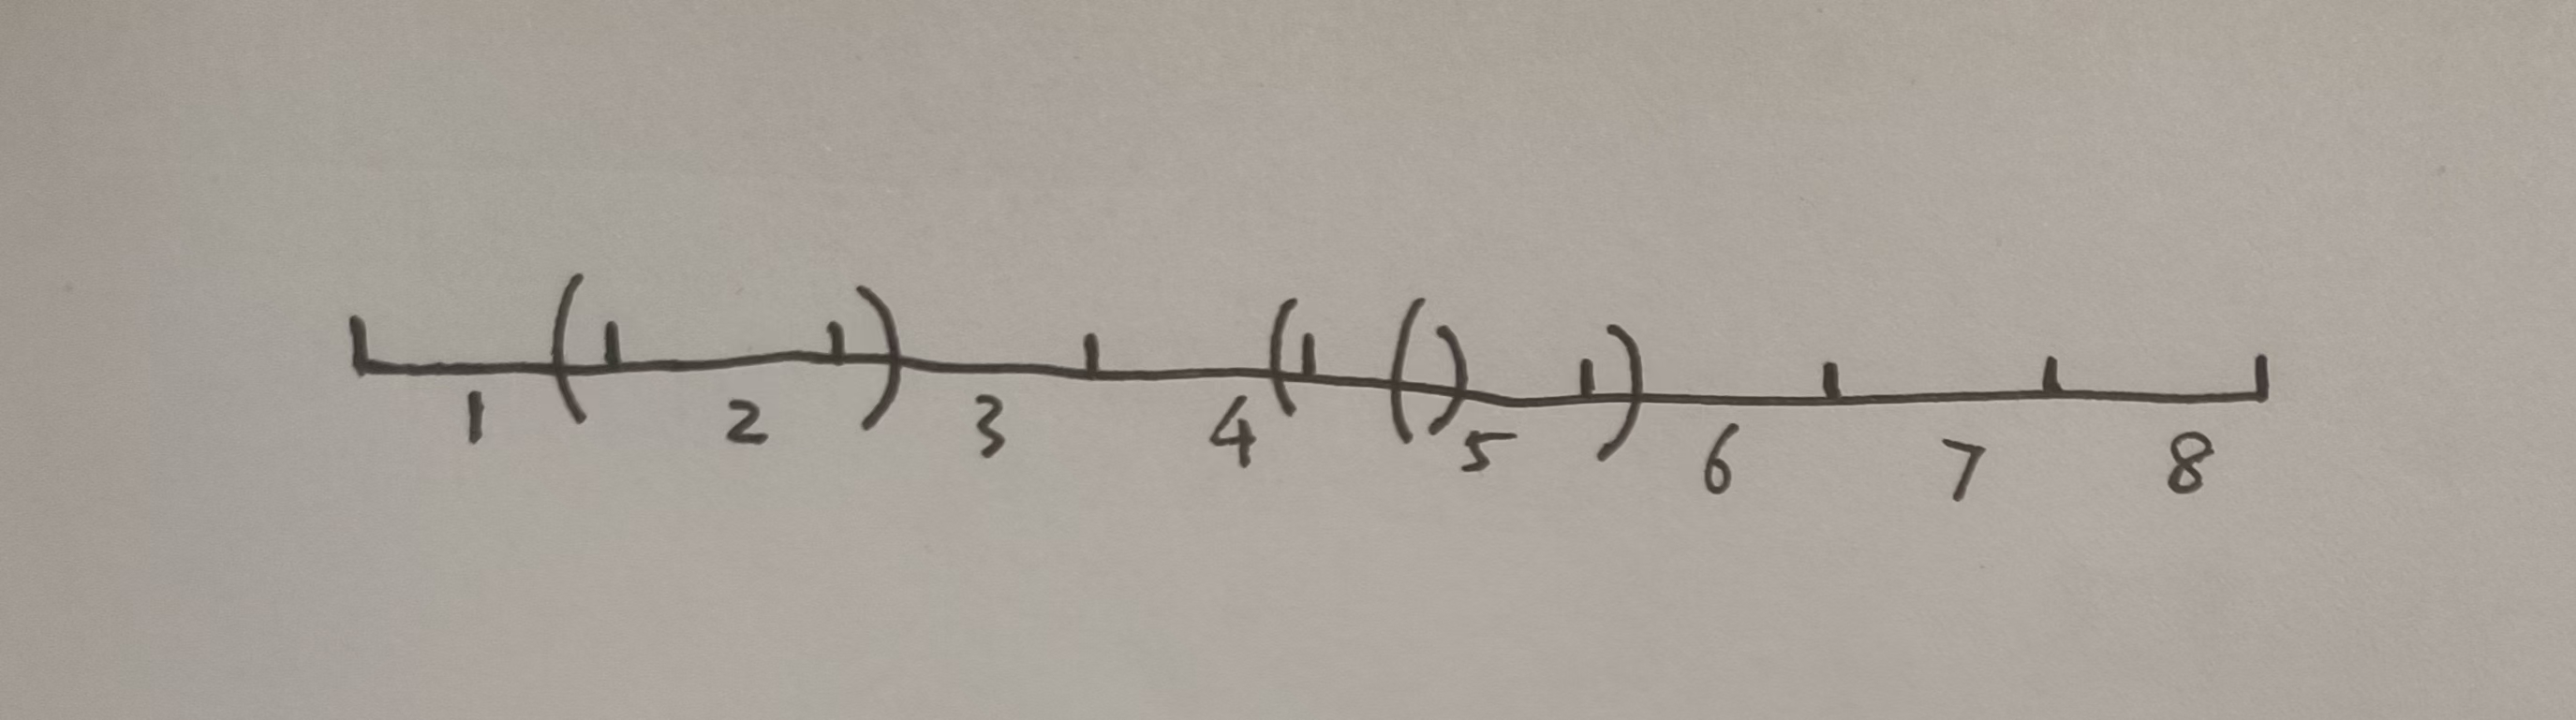
\includegraphics[width=0.6\textwidth]{figs_P1/1.jpg}
    \caption{Your imagination}
    \label{fig:yours}
\end{figure}
where the parentheses are those open intervals in $\mathcal{J}$, and $\Delta x_j$ just involves the subintervals 1, 2, 3, 4, 5 and 6, and the exceeding part of $\sum_j \Delta x_j$ than $\mathcal{J}$ are the subintervals 1,3,4 and 6, which would vanish as the segmentation grows denser. But here $\mathcal{J}$ has too few intervals, and it does fail if, say, $D(f)$ is the set of all rational numbers in $[a,b]$. This case whatever $\mathcal{J}$ and $\pmb{\pi}$ are like, the $\Delta x_j$ always involves all the subintervals from the segmentation, due to the density of the rational numbers.

The solution from the reference book is to, say, let $\Delta x_j$ includes the subintervals 2 and 5 here so that $\sum_j \Delta x_j \leq |\mathcal{J}|$, and let those ``marginal'' subintervals 1,3,4 and 6 be included in $\sum_i \Delta x_i$. Since the subintervals 1,3,4,6 may contain some discontinuity, the following lemma is proposed to extend the uniform continuity of $f$.

\begin{Th}{Lma 7\_P1.1.5.7}
    Suppose $f$ is a real function defined on $[a,b]$. Let the set $D(f)$ of discontinuous points of $f$ is covered by a sequence $\mathcal{J}$ of open intervals, and denote $K = [a,b]\setminus \mathcal{J}$. Then for any $\varepsilon > 0$, there exist a $\delta > 0$ such that for any $x\in K$ and $y\in [a,b]$ with $|x-y|<\delta$, we have $|f(x)-f(y)|<\varepsilon$.
    \tcblower
    \textit{Pf}: The proof is similar to the previous one for the uniform continuity. If otherwise, then there exist an $\varepsilon_0 > 0$, and two sequences $\{x_n\}$ in $K$ and $\{y_n\}$ in $[a,b]$, with $|x_n-y_n|<1/n$ and $|f(x_n)-f(y_n)|\geq \varepsilon_0$. Say $\lim\limits_{n\to\infty} x_n = \lim\limits_{n\to\infty} y_n = x$ (otherwise there are anyway respective convergent subsequences). Since $x_n\in K$, by the closedness of $K$ (and hence sequence-compactness), $x\in K$. And $f$ is continuous at $x$, so that $\lim\limits_{n\to\infty} f(x_n) = f(x) = \lim\limits_{n\to\infty} f(y_n)$, contradicting $|f(x_n)-f(y_n)|\geq \varepsilon_0$.
\end{Th}

With this lemma, the subintervals 1,3,4,6, namely, those containing the points from both $K$ and $\mathcal{J}$, can be perfectly limited by $\Vert \pmb{\pi} \Vert$. 

Lastly there is a detail: to strictly state that $\sum_j \Delta x_j \leq |\mathcal{J}|$. Since by the finite-covering theorem, it holds if $\Delta x_j$ includes only one closed interval, this statement becomes natural if we simply join the finite number of closed intervals $\Delta x_j$'s to form a single closed interval, moving the ``coverers'' of $\mathcal{J}$ correspondingly. Then all the details prepared, please write down the obvious formal proof by yourself.

\begin{Df}{Df 7\_P1.1.5.8 (almost everywhere / a.e.)}
    For a property $P(x)$ about $x\in A\subseteq\mathbb{R}$, we say that $P(x)$ holds \textbf{almost everywhere (a.e.)} on $A$ if the set of points $x\in A$ where $P(x)$ fails is of measure zero.
\end{Df}

\begin{Th}{Th 7\_P1.1.5.9 (Lebesgue criterion)}
    Suppose $f$ is a real function defined on $[a,b]$. Then $f$ is integrable on $[a,b]$ iff $f$ is continuous almost everywhere on $[a,b]$.
\end{Th}

Note that the ``integrable'' here is in the sense of the Riemann integral. All the way here we realize that the Riemann's integral is specially designed for the continuous functions. Instead, Lebesgue loosened the requirement and proposed the Lebesgue integral, whose discussion is left to the course \textbf{real analysis}.
\end{document}